\let\lesson\undefined
\newcommand{\lesson}{\phantomlesson{Bài 9.}}
\setcounter{section}{2}
\section{Bài tập trắc nghiệm}
\begin{enumerate}[label=\bfseries Câu \arabic*:,leftmargin=1.5cm]
	\item \mkstar{1}\\
	{Một vật ném xiên có quỹ đạo như hình vẽ. Tầm bay xa của vật là khoảng cách giữa
		\begin{center}
			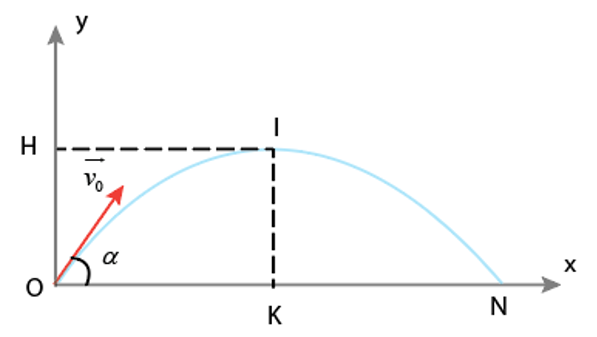
\includegraphics[width=0.4\linewidth]{../figs/VN10-2022-PH-TP013-P-1}
		\end{center}
	\begin{mcq}
		\item điểm ném và điểm cao nhất của quỹ đạo.
		\item điểm cao nhất của quỹ đạo và điểm rơi.
		\item điểm cao nhất của quỹ đạo và điểm có gia tốc bằng 0.
		\item điểm ném và điểm rơi trên mặt đất.
	\end{mcq}
}
\hideall{
\textbf{Đáp án: D.}
}

\item \mkstar{1}\\
{Một quả tạ được ném từ độ cao $h$ sao cho vận tốc ban đầu $\overrightarrow{v_0}$ hợp với phương ngang một góc $\alpha$. Tầm xa của quả tạ phụ thuộc vào
	\begin{mcq}(2)
		\item góc ném $\alpha$ và vận tốc ban đầu $v_0$.
		\item lực cản của không khí.
		\item độ cao $h$.
		\item tất cả các yếu tố trên.
	\end{mcq}

}
\hideall{
\textbf{Đáp án: D.}
}

\item \mkstar{1}\\
{Một vật ném xiên có quỹ đạo như hình vẽ. Tầm cao của vật ném xiên là đoạn
\begin{center}
	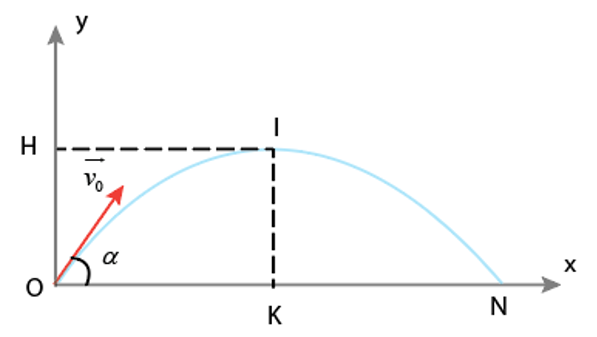
\includegraphics[width=0.4\linewidth]{../figs/VN10-2022-PH-TP013-P-1}
\end{center}
\begin{mcq}(4)
	\item IK.
	\item OI.
	\item OK.
	\item NO
\end{mcq}
}
\hideall{
\textbf{Đáp án: A.}
}

\item \mkstar{2}\\
{Trong hình vẽ sau, gia tốc của vật tại đỉnh I có
	\begin{center}
		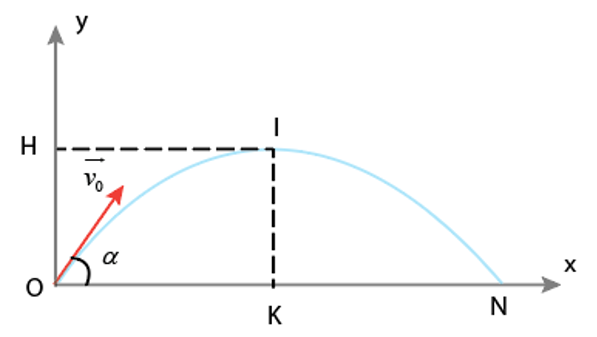
\includegraphics[width=0.4\linewidth]{../figs/VN10-2022-PH-TP013-P-2}
	\end{center}
\begin{mcq}(2)
	\item hướng ngang theo chiều từ H đến I.
	\item hướng ngang theo chiều từ I đến H.
	\item hướng thẳng đứng xuống dưới.
	\item hướng thẳng đứng lên trên.
\end{mcq}
}
\hideall{
\textbf{Đáp án: C.}
}

\item \mkstar{3}\\
{Một vật được ném xiên từ mặt đất lên với vận tốc ban đầu là $v_0 = \SI{10}{\meter/\second}$ theo phương hợp với phương nằm ngang góc $\SI{30}{\degree}$. Lấy $g = \SI{10}{\meter/\second^2}$. Độ cao cực đại và tầm xa mà vật đạt được lần lượt là
	\begin{mcq}(4)
		\item $\SI{1.25}{\meter}$; $\SI{8.66}{\meter}$.
		\item $\SI{8.66}{\meter}$; $\SI{1.25}{\meter}$.
		\item $\SI{1.25}{\meter}$; $\SI{22.5}{\meter}$.
		\item $\SI{22.5}{\meter}$; $\SI{8.66}{\meter}$.
	\end{mcq}

}
\hideall{
\textbf{Đáp án: A.}\\
Độ cao cực đại mà vật đạt được:
$$H=\dfrac{v^2_0\sin^2\theta}{2g}=\SI{1.25}{\meter}$$
Tầm xa mà vật đạt được:
$$L=\dfrac{v^2_0\sin2\theta}{g}=\SI{8.66}{\meter}.$$
}

\item \mkstar{3}\\
{Một vật được ném lên từ mặt đất theo phương xiên góc hợp với phương ngang một góc $\alpha =\SI{45}{\degree}$, với vận tốc ban đầu là $\SI{5}{\meter/\second}$. Bỏ qua mọi lực cản. Lấy $g = \SI{10}{\meter/\second^2}$. Độ cao cực đại của vật là
\begin{mcq}(4)
	\item $\SI{0.25}{\meter}$.
	\item $\SI{0.5}{\meter}$.
	\item $\SI{0.625}{\meter}$.
	\item $\SI{1.25}{\meter}$.
\end{mcq}
}
\hideall{
\textbf{Đáp án: C.}\\
Độ cao cực đại mà vật đạt được:
$$H=\dfrac{v^2_0\sin^2\theta}{2g}=\SI{0.625}{\meter}.$$
}

\item  \mkstar{3}\\
{Một vật được ném với vận tốc $\SI{12}{\meter/\second}$  với góc ném $\alpha=\SI{30}{\degree}$ so với mặt phẳng nằm ngang. Lấy $g = \SI{10}{\meter/\second^2}$. Hòn đá rơi đến đất cách chỗ ném theo phương ngang một khoảng $\SI{200}{\meter}$. Thời gian vật rơi là
\begin{mcq}(4)
	\item $\SI{24.5}{\second}$.
	\item $\SI{19.2}{\second}$.
	\item $\SI{14.6}{\second}$.
	\item $\SI{32.8}{\second}$.
\end{mcq}
}
\hideall{
\textbf{Đáp án: B.}\\
\textit{Lưu ý: Sửa đề lại, vật được ném từ vị trí bất kì, không phải ném từ mặt đất.}
Thời gian vật rơi:
$$t=\dfrac{L}{v_0\cos\alpha}=\SI{19.2}{\second}.$$

}

\item \mkstar{3}\\
{Một vật được ném lên từ mặt đất theo phương xiên góc hợp với phương ngang một góc $\alpha$. Khi lên đến độ cao cực đại cách mặt đất $\SI{15}{\meter}$ thì vận tốc bằng một nửa vận tốc ban đầu. Lấy $g =\SI{10}{\meter/\second^2}$. Tính độ lớn vận tốc ban đầu.
	\begin{mcq}(4)
		\item $\SI{18}{\meter/\second}$.
		\item $\SI{20}{\meter/\second}$.
		\item $\SI{15}{\meter/\second}$.
		\item $\SI{25}{\meter/\second}$.
	\end{mcq}

}
\hideall{
\textbf{Đáp án: B.}\\
Khi vật lên đến độ cao cực đại:
$$v_x=v_0\cos\alpha; v_y=0\Rightarrow v=v_0\cos\alpha$$
Mà lúc này $v=\dfrac{v_0}{2}\Rightarrow \cos\alpha=\dfrac{1}{2}\Rightarrow \alpha=\SI{60}{\degree}$.\\
Độ cao cực đại vật đạt được:
$$H=\dfrac{v^2_0\sin^2\alpha}{2g}\Rightarrow v_0=\SI{20}{\meter/\second}.$$
}

\item \mkstar{4}\\
{Từ độ cao $\SI{7.5}{\meter}$ người ta ném một quả cầu với vận tốc ban đầu $\SI{10}{\meter/\second}$, ném xiên góc $\SI{45}{\degree}$ so với phương ngang. Vật chạm đất tại vị trí cách vị trí ban đầu theo phương nằm ngang một khoảng bằng
	\begin{mcq}(4)
		\item $\SI{5}{\meter}$.
		\item $\SI{15}{\meter}$.
		\item $\SI{9}{\meter}$.
		\item $\SI{18}{\meter}$.
	\end{mcq}

}
\hideall{
\textbf{Đáp án: B.}\\
Chọn gốc toạ độ $O$ tại mặt đất, trục $Oy$ thẳng đứng hướng lên, trục $Ox$ cùng hướng chuyển động của vật trên phương ngang. Gốc thời gian trùng lúc ném vật.\\
Phương trình chuyển động của vật trên phương thẳng đứng:
$$y=h_0+v_0\sin\theta t-\dfrac{1}{2}\cdot gt^2=7,5+5\sqrt{2}t-5t^2$$
Khi vật chạm đất thì $y=0\Rightarrow t=\xsi{1,5\sqrt{2}}{\second}$.\\
Tầm xa của vật:
$$L=v_0\cos\alpha\cdot t=\SI{15}{\meter}.$$
}

\item \mkstar{4}\\
{Từ một đỉnh tháp cao $\SI{12}{\meter}$ so với mặt đất, người ta ném một hòn đá với vận tốc ban đầu $v_0=\SI{15}{\meter/\second}$, theo phương hợp với phương nằm ngang một góc $\alpha=\SI{45}{\degree}$. Khi chạm đất, hòn đá có tốc độ bằng bao nhiêu? Lấy $g = \SI{9.8}{\meter/\second^2}$.
\begin{mcq}(4)
	\item $\SI{18.6}{\meter/\second}$.
	\item $\SI{24.2}{\meter/\second}$.
	\item $\SI{28.8}{\meter/\second}$.
	\item $\SI{21.4}{\meter/\second}$.
\end{mcq}
}
\hideall{
\textbf{Đáp án: D.}\\
Chọn gốc toạ độ $O$ tại mặt đất, trục $Oy$ thẳng đứng hướng lên, trục $Ox$ cùng hướng chuyển động của vật trên phương ngang. Gốc thời gian trùng lúc ném vật.\\
Phương trình vận tốc của hòn đá trên 2 phương $Ox$ và $Oy$:
\begin{align*}
	\begin{cases}
		v_x=v_0\cos\alpha\\
		v_y=v_0\sin\alpha-gt
	\end{cases}
\end{align*}
Phương trình chuyển động của hòn đá trên phương thẳng đứng:
$$y=h_0+v_0\sin\left(\alpha\right)t-\dfrac{1}{2}gt^2=12+7,5\sqrt{2}t-4,9t^2$$
Khi hòn đá chạm đất thì $y=0\Rightarrow t\approx\SI{2.985}{\second}$\\
Vận tốc của vật trên hai phương $Ox$ và $Oy$ lúc này:
\begin{align*}
	\begin{cases}
		v_x=\xsi{7,5\sqrt{2}}{\meter/\second}\\
		v_y\approx\SI{-18.65}{\meter/\second}
	\end{cases}
\end{align*}
Tốc độ của vật khi chạm đất:
$$v=\sqrt{v^2_x+v^2_y}\approx\SI{21.45}{\meter/\second}.$$
}
\end{enumerate}
\section{Bài tập tự luận}
\begin{enumerate}[label=\bfseries Bài \arabic*:,leftmargin=1.5cm]
	\item \mkstar{3}
	
	
	{Một vật ném xiên góc $45^\circ$ từ mặt đất và rơi cách đó $\SI{30}{m}$. Tính vận tốc khi ném, lấy $g=\SI{10}{m/s}^2$.
	}
	
	\hideall
	{	
		
		Vận tốc khi bị ném
		
		$$L = \dfrac{v^2_0 \sin 2\alpha}{g} = 30 \Rightarrow v_0 = \xsi{10\sqrt 3}{m/s}.$$
	}
	
	
	\item \mkstar{3}
	
	
	{Vật được ném xiên góc $60^\circ$ với vận tốc $\SI{30}{m/s}$, lấy $g=\SI{10}{m/s}^2$, tính tầm xa và độ cao cực đại vật đạt được.
	}
	
	\hideall
	{	
		Tầm xa của vật
		
		$$L = \dfrac{v^2_0 \sin 2\alpha}{g} = \SI{77,94}{m}.$$
		
		Độ cao cực đại
		
		$$H = \dfrac{v^2_0\sin^2 2\alpha}{2g} = \SI{33,75}{m}.$$
		
	}
	\item \mkstar{3}
	
	
	
	{Ném xiên góc $45^\circ$ một vật với vận tốc $\SI{25}{m/s}$. Lấy $g=\SI{10}{m/s}^2$, tính vận tốc của vật sau khi ném $\SI{1,2}{s}$.
	}
	
	\hideall
	{	
		Ta có:
		
		$$\begin{cases}
			v_\text{x} = v_0 \cos \alpha = \SI{17,677}{m/s}.\\
			v_\text{y} = v_0 \sin \alpha - gt = \SI{5,677}{m/s}.
		\end{cases}$$
		
		Vận tốc của vật
		
		$$v = \sqrt{v^2_\text{x} + v^2_\text{y}} = \SI{18,6}{m/s}.$$
		
	}
	\item \mkstar{3}
	
	
	
	{Từ mặt đất một vật được ném xiên với phương ngang một góc $\alpha = 45^\circ$ với vận tốc ban đầu là $\SI{20}{m/s}$. Lấy $g=\SI{10}{m/s}^2$. Viết phương trình chuyển động, phương trình quỹ đạo của vật và độ cao mà vật có thể lên tới.
	}
	
	\hideall
	{	
		
		\begin{center}
			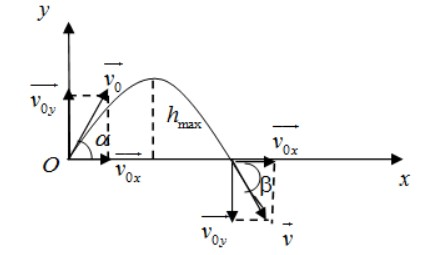
\includegraphics[scale=1.2]{../figs/VN10-2021-PH-TP014-2.jpg}
		\end{center}
	Chọn gốc toạ độ tại vị trí ném, trục $Oy$ thẳng đứng hướng lên, trục $Ox$ cùng hướng chuyển động của vật trên phương nằm ngang. Gốc thời gian trùng thời điểm ném.
	
	Phương trình vận tốc của vật:
	\begin{align*}
		\begin{cases}
			v_x=v_0\cos\alpha=10\sqrt{2}\quad\left(\si{\meter/\second}\right)\\
			v_y=v_0\sin\alpha-gt=10\sqrt{2}-10t\quad\left(\si{\meter/\second}\right)
		\end{cases}
	\end{align*}
	Phương trình chuyển động của vật:
	\begin{align*}
		\begin{cases}
			x=v_0t\cos\alpha=10\sqrt{2}t\quad\left(\si{\meter}\right)\\
			y=v_0t\sin\alpha -\dfrac{1}{2}\cdot gt^2=10\sqrt{2}t-5t^2\quad\left(\si{\meter}\right)
		\end{cases}
	\end{align*}
Phương trình quỹ đạo của vật:
$$y=x-\dfrac{x^2}{40}$$
Khi vật lên đến độ cao cực đại thì $v_y=0\Rightarrow t=\xsi{\sqrt{2}}{\second}$.\\
Độ cao cực đại của vật
$$y_\text{max}=\SI{10}{\meter}.$$
	}
\item \mkstar{4}


{Từ A (độ cao AC = $H$ = $\SI{3,6}{m}$) người ta thả một vật rơi tự do, cùng lúc đó từ B cách C đoạn BC = $L$ = $H$ người ta ném một vật khác với vận tốc ban đầu $v_0$ hợp với phương ngang góc $\alpha$. Tính $\alpha$ và $v_0$ để hai vật gặp được nhau khi vật A qua vị trí bằng 1 nửa độ cao ban đầu. Lấy gia tốc rơi tự do $g=\SI{10}{\meter/\second^2}$.
	
	\begin{center}
		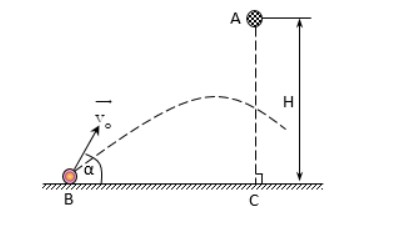
\includegraphics[scale=1]{../figs/VN10-2021-PH-TP014-1.jpg}
	\end{center} 
}

\hideall
{	Chọn gốc toạ độ tại C, trục $Oy$ thẳng đứng hướng lên, trục $Ox$ hướng từ B sang C.
	
	Phương trình chuyển động của vật thả rơi (vật I):
	
	$$x_1 = 0; y_1 = H -\text{0,5}gt^2.$$
	
	Phương trình chuyển động của vật II:
	
	$$\begin{cases}
		x_2 = L  - (v_0 \cos \alpha)t = H - (v_0\cos \alpha)t.\\
		y_2 = (v_0\sin \alpha) t - \text{0,5}gt^2.
	\end{cases}$$
	
	Để hai vật gặp nhau $x_1 = x_2$ và $y_1 = y_2$
	
	$$\begin{cases}
		(v_0\cos \alpha) t = H.\\
		(v_0 \sin \alpha)t = H.
	\end{cases} \Rightarrow \tan \alpha = 1 \Rightarrow \alpha = \SI{45}{\degree}$$
	
	Nhân 2 vế của hệ phương trình trên với nhau ta được
	$$v^2_0\cdot\dfrac{\sin2\alpha}{2}\cdot t^2=H^2 \Rightarrow v_0=\dfrac{H\sqrt{2}}{t\sqrt{\sin2\alpha}}$$
	
	Mà hai vật gặp nhau tại vị trí $y_1=\dfrac{H}{2}\Rightarrow t=\sqrt{\dfrac{H}{g}}\Rightarrow v_0=\sqrt{\dfrac{2Hg}{\sin 2\alpha}} = \xsi{6\sqrt{2}}{m/s}.$
}
\end{enumerate}
